\begin{figure}[htbp]
    \captionsetup[subfigure]{justification=centering}
    \centering
    \begin{subfigure}[b]{0.28\textwidth}
        \centering
        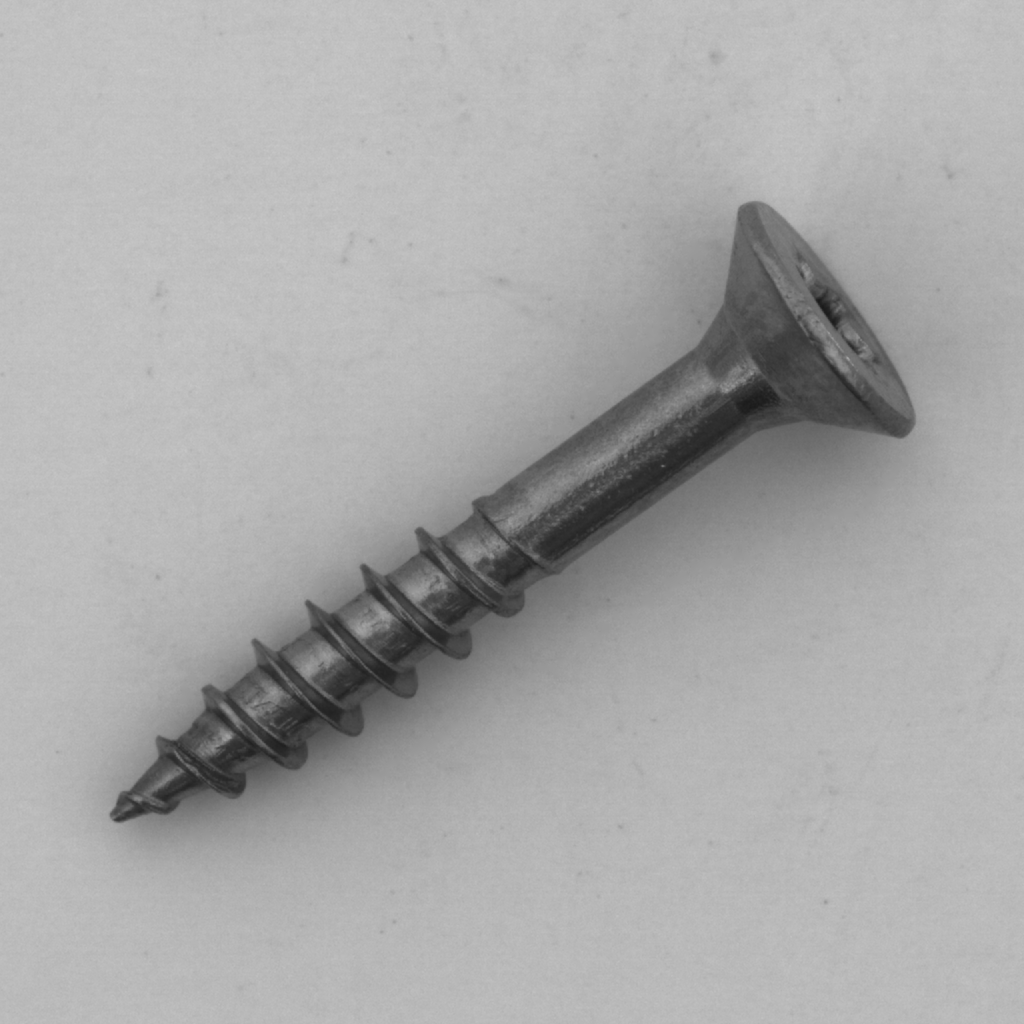
\includegraphics[width=\textwidth]{figures/introductionanomalies/033.png}
        %\caption*{original Image}

    \end{subfigure}
    \hspace{0.05\textwidth} % Add space between subfigures
    \begin{subfigure}[b]{0.28\textwidth}
        \centering
        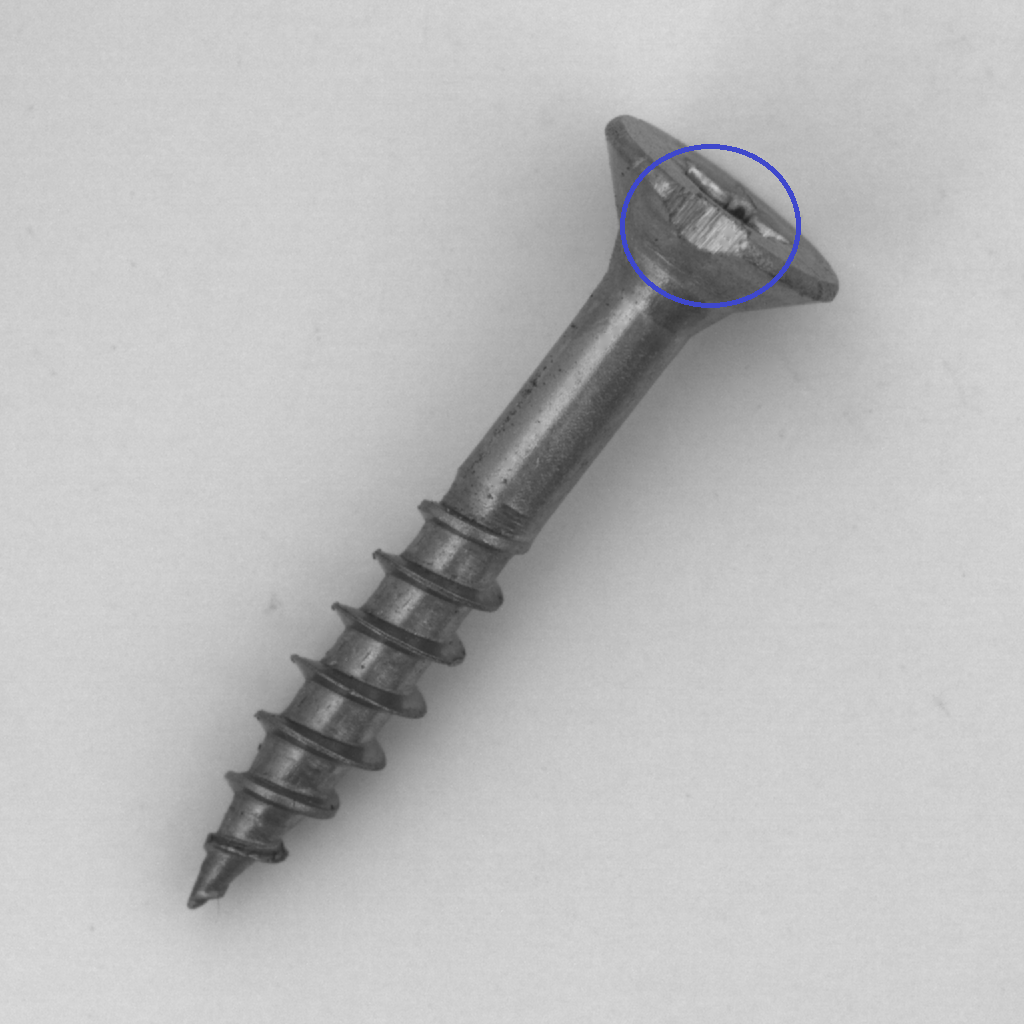
\includegraphics[width=\textwidth]{figures/introductionanomalies/manifrontcopy.png}
        %\caption*{Mask}

    \end{subfigure}
    \hspace{0.05\textwidth} % Add space between subfigures
    \begin{subfigure}[b]{0.28\textwidth}
        \centering
        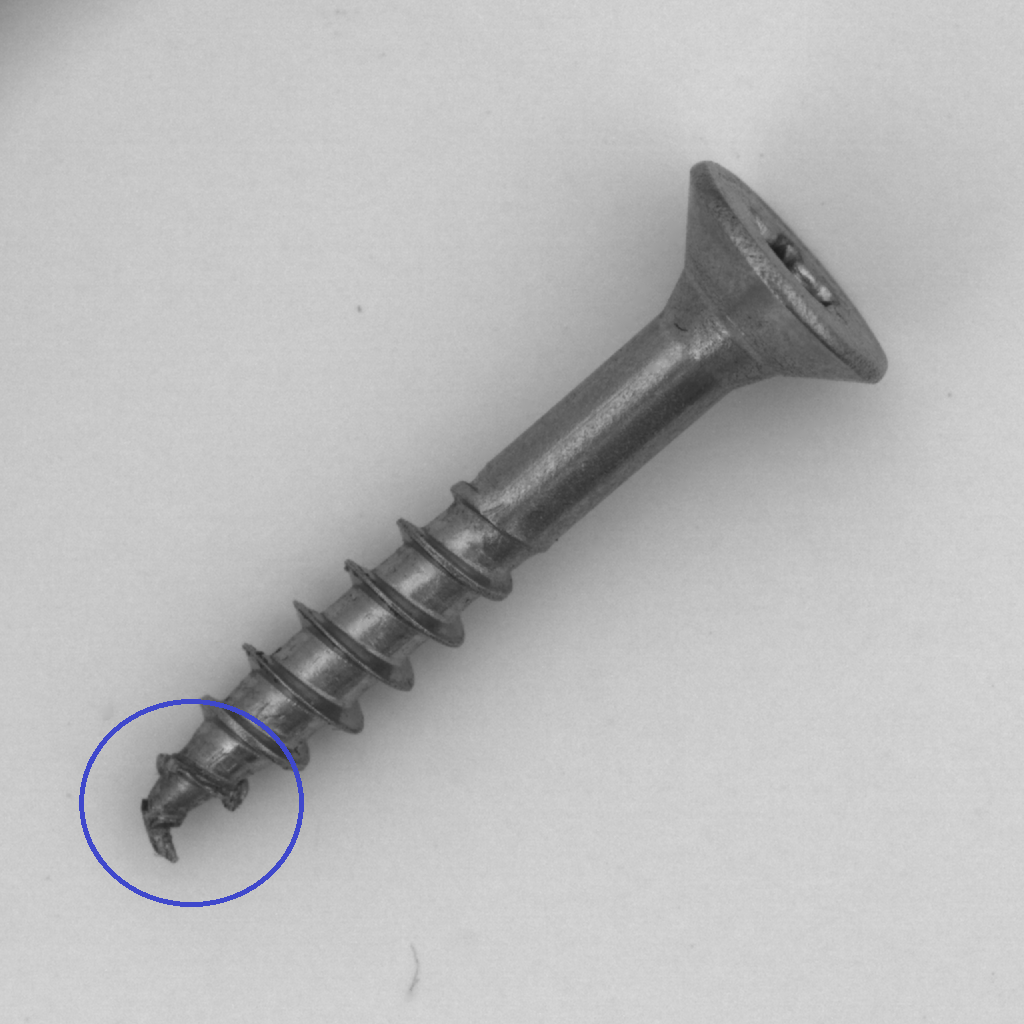
\includegraphics[width=\textwidth]{figures/introductionanomalies/realfrontnow.png}
        %\caption*{Discriminator Predictions}

    \end{subfigure}
    \caption{Instance images of a screw from \cite{MVTEC_Bergmann_2021} to showcase anomalous objects in manufacturing settings. The images include a regular screw, a screw with a chipped head and a screw with a bent tip.}
    \label{fig:introscrew}
\end{figure}